\chapter{Chapitre 1: Etude préalable}
\begin{spacing}{1.2}
\minitoc
\thispagestyle{MyStyle}
\end{spacing}
\newpage
\renewcommand{\tablename}{Tableau}
\begin{sloppypar} 

\section{Introduction }
\vspace{-4mm}
Ce chapitre vise à situer le projet dans son contexte général. Nous débutons en présentant l'entreprise d'accueil, InfoBjectif. Ensuite, nous identifions la problématique et définissons le contexte global pour positionner le projet dans son environnement organisationnel, méthodologique et stratégique. Nous terminons en critiquant l'état actuel des choses, en présentant la solution proposée et la méthodologie à suivre, ainsi que la gestion du temps pour les différentes tâches du projet sous la forme d'un diagramme de Gantt. 
\vspace{-6mm}
\section{Organisme d’accueil  }
\vspace{-4mm}
InfoBjectif est une entreprise de Services en Ingénierie Informatique (SSII) . Nous débutons cette section en présentant InfoBjectif, et concluons en exposant l'organigramme de l'équipe au sein de laquelle j’ai effectué mon stage de fin d'études .
\vspace{-6mm}
\subsection{Présentation de Infobjectif}
\vspace{-4mm}
\subsubsection{Introduction}
\vspace{-4mm}
Infobjectif se positionne comme un acteur majeur dans le domaine de la transformation numérique sur le marché tunisien. L'entreprise offre une gamme complète de services, incluant le conseil, l'intégration de systèmes, le déploiement de solutions métiers, la gestion d'infrastructure et des services de processus d'entreprise. Cette diversité de services permet aux grandes entreprises de relever les défis liés au développement et à la compétitivité dans un environnement numérique en constante évolution.

\begin{figure}[H]%
    \center%
    \setlength{\fboxsep}{5pt}%
    \setlength{\fboxrule}{0.5pt}%
    \fbox{
    
\includegraphics[width=5cm]{images/InfoLogo.png}%
    }
    \caption{Logo Infobjectif}%
\end{figure}

\subsubsection{Coordonnées de l'entreprise}

\begin{flushleft}
\textbf{Adresse:} Tunis, Rue Nijer \\
\textbf{Téléphone:} 23236236 \\
\textbf{Adresse e-mail:} infoobjectif@gmail.com
\end{flushleft}

\subsection{Organigramme de la societé}
\vspace{-4mm}
la figure 1.2 présente l'organigramme de la societé : 
\begin{figure}[H]%
    \center%
    \setlength{\fboxsep}{5pt}%
    \setlength{\fboxrule}{0.5pt}%
    \fbox{
    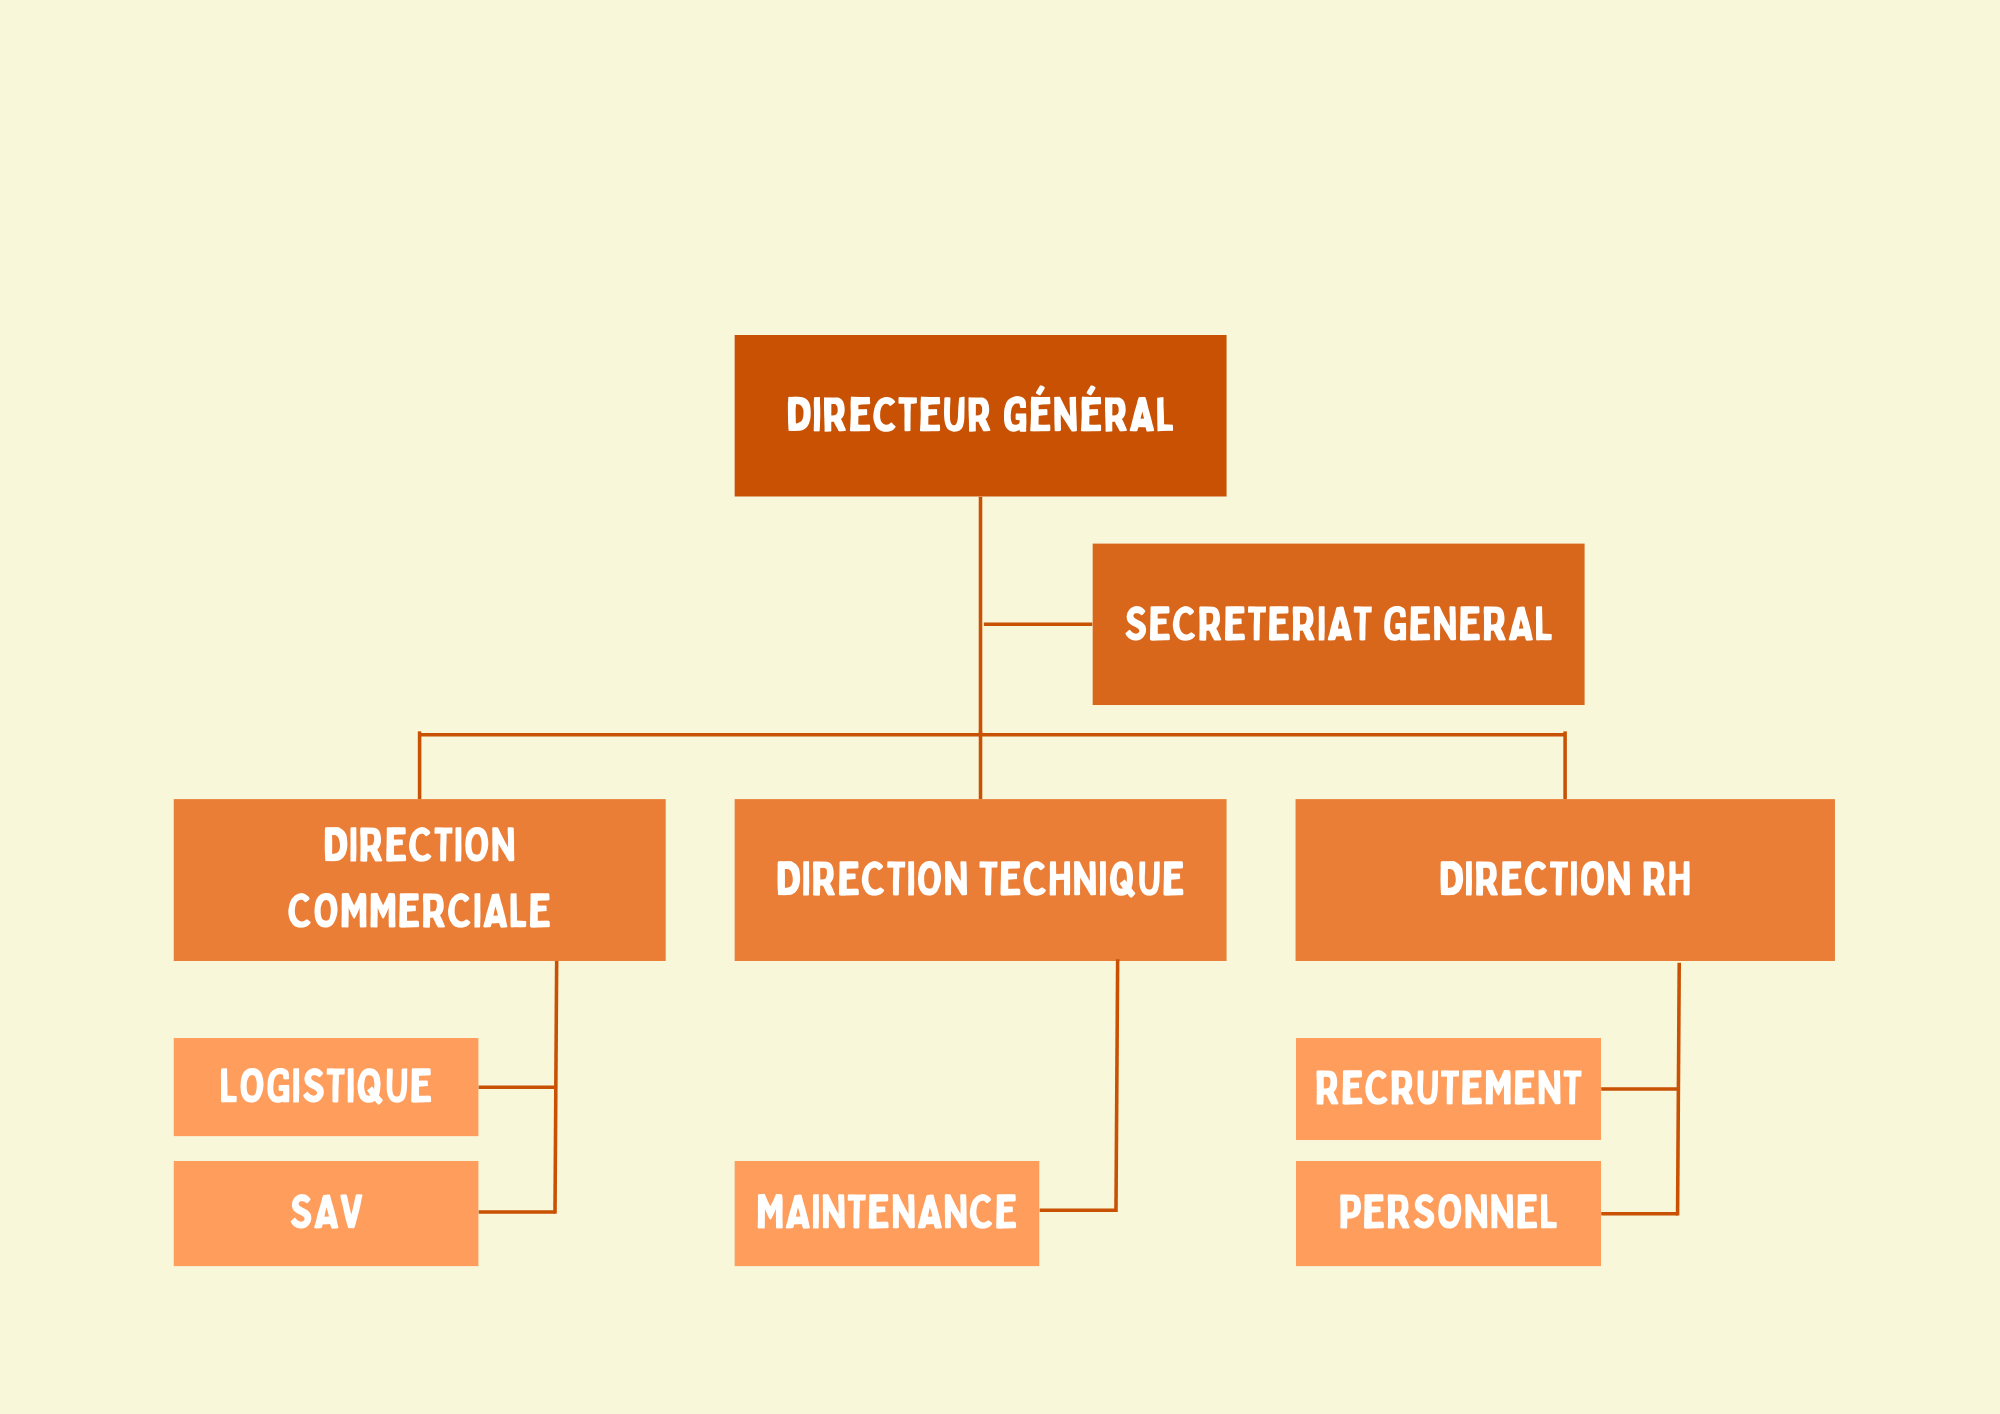
\includegraphics[width=15cm]{images/Organigramme infobjectif.png}%
    }
    \caption{Organigramme de L'entreprise}%
\end{figure}
\vspace{-15mm}
\section{Présentation du projet}
\vspace{-6mm}
\subsection{Contexte du projet}
\vspace{-4mm}
Nous avons pour mission dans le cadre de notre projet de fin d'études en vue de l’obtention de la Licence Appliquée en Technologie de L’Informatique DSI.
Il consiste à la conception et le développement d’une application web et mobile  de gestion
des services pour les etudians et de communication 
une période de 14 semaines.

\vspace{-9mm}
\subsection{Etude de l’existant }
\vspace{-4mm}
L'étude de l'existant met en évidence les différents systèmes et pratiques actuels utilisés par les étudiants pour accéder aux informations universitaires et communiquer avec l'administration. Actuellement, les informations importantes, telles que les événements sur le campus et les offres de stage, sont disponibles sur divers supports, y compris les sites web, les panneaux d'affichage et les réseaux sociaux. Chaque support contient des informations spécifiques, nécessitant souvent des recherches sur plusieurs plateformes pour obtenir une vue d'ensemble complète. De plus, il y a une dispersion des informations sans centralisation claire, ce qui peut augmenter le temps nécessaire pour trouver des informations précises. Les outils actuels manquent de fonctionnalités avancées de filtrage et de personnalisation, ce qui rend la recherche d'informations spécifiques plus complexe. Ces observations montrent l'opportunité de développer une solution numérique centralisée pour améliorer l'accès aux informations et la communication au sein de l'université.
\vspace{-6mm}
\subsection{Critique de l’existant }
\vspace{-4mm}
La fragmentation de l'information est un problème clé, avec des données cruciales dispersées sur divers supports tels que les sites web, les panneaux d’affichage et les réseaux sociaux, compliquant ainsi l'accès rapide et efficace aux informations nécessaires. Cette dispersion entraîne également un manque de centralisation, obligeant les étudiants à rechercher les mêmes informations sur plusieurs plateformes, ce qui conduit à une perte de temps considérable. De plus, les canaux de communication existants sont inefficaces et ne répondent pas adéquatement aux besoins des étudiants, rendant difficile l'interaction rapide et efficace avec l'administration universitaire. Enfin, l'absence de fonctionnalités de filtrage et de personnalisation complique encore davantage la recherche d’informations, empêchant les étudiants de trouver facilement les informations les plus pertinentes pour eux.
\vspace{-6mm}
\section{Solution proposée}
\vspace{-4mm}
\adjustmtc
\thispagestyle{MyStyle}
\vspace{-4mm}
Pour répondre aux défis rencontrés par les étudiants dans leur recherche d’informations pertinentes et leur communication avec l’administration universitaire, nous proposons la mise en place d’une solution numérique centralisée et efficace. Cette solution permettra de regrouper toutes les données dispersées sur différents supports tels que les sites web, les panneaux d’affichage et les réseaux sociaux. En centralisant ces informations, nous offrirons aux étudiants un accès simplifié et rapide à toutes les données dont ils ont besoin. De plus, notre solution comprendra des fonctionnalités avancées de filtrage et de personnalisation, permettant à chaque utilisateur de trouver facilement les informations pertinentes tout en réduisant considérablement le temps nécessaire à leur recherche.

Pour résoudre ces problèmes, notre solution centralise à :
\begin{itemize}
    \item Rassembler toutes les informations dispersées sur divers supports au sein d'une plateforme numérique unique pour un accès unifié et fiable.
    \item Intégrer des options avancées de filtrage permettant aux étudiants de sélectionner et d'afficher uniquement les informations pertinentes selon leurs besoins spécifiques.
    \item Intégrer des outils de communication efficaces comme des messageries instantanées pour faciliter les échanges entre étudiants et administration, améliorant ainsi la résolution rapide des problèmes et la réponse aux questions en temps réel.
\end{itemize}

Cette approche vise à optimiser l'expérience des étudiants en leur fournissant un accès facile et structuré aux informations essentielles, tout en améliorant l'efficacité globale de la communication au sein de l'université.

\vspace{-6mm}
\section{Méthodologie du travail }
\vspace{-4mm}
La méthodologie du travail pour la réalisation de cette solution numérique, peut être décomposée en plusieurs étapes clés :

\underline{\textbf{Analyse des besoins : }} Comprendre en profondeur les besoins des étudiants et des administrateurs universitaires en termes d'informations, de communication et d'interactions. Cela implique des entretiens avec les parties prenantes, des sondages et des études de marché pour identifier les fonctionnalités et les exigences essentielles de la plateforme.

\underline{\textbf{Conception de l'architecture :}} Concevoir une architecture logicielle robuste qui prend en charge les fonctionnalités souhaitées tout en garantissant la scalabilité, la performance et la sécurité. Cette étape comprend également la définition des interfaces utilisateur et des flux de navigation pour une expérience utilisateur optimale.

\underline{\textbf{Développement frontend : }} Développement d'une application mobile destinée aux étudiants, et la conception d'une interface d'administration web. L'accent sera mis sur la création d'interfaces utilisateur intuitives et faciles à utiliser, avec une navigation fluide et des fonctionnalités accessibles, pour assurer une expérience utilisateur optimale.

\underline{\textbf{Développement backend : }}Implémentation du backend de l'application pour gérer efficacement les requêtes des utilisateurs et assurer la gestion optimale des données. Cette phase inclut la création de services pour répondre aux besoins fonctionnels de l'application et la mise en place d'une infrastructure de base de données pour le stockage sécurisé des informations essentielles.


\underline{\textbf{Intégration continue et déploiement : }} Mettre en place des pipelines d'intégration continue pour automatiser les tests et les déploiements, assurant ainsi la qualité du code et la stabilité de l'application tout au long du processus de développement. Utiliser des outils tels que Jenkins, GitLab CI ou GitHub Actions pour cette tâche.

\vspace{-6mm}
 \subsection{UP (Processus Unifié) }
 \vspace{-4mm}
 Le processus unifié est une méthode d’implémentation et de développement, majoritairement utilisée par les développeurs informatiques. Il s’agit d’un processus itératif et implémentable. Il est caractérisé par quatre aspects : 
\\1.	Un pilotage par les cas d’utilisation 
\\2.	L’architecture au cœur du processus
\\3.	L’utilisation maximale des modèles, plus spécifiquement des modèles UML 
\\4.	La levée régulière des incertitudes grâce à sa dimension itérative et cyclique [1].
\vspace{-6mm}
\subsection{SCRUM : Agile}
\vspace{-4mm}
La méthode SCRUM définit un cadre de travail permettant la réalisation de projets complexes. Initialement prévu pour le développement de projets type « Software », cette méthode peut être appliquée à tout type de projet, du plus simple au plus innovant, et ce de manière très simple. Cette méthodologie permet de s’adapter rapidement aux changements du client à fréquence régulière. Chaque fin d'itération, l'équipe et le client réévaluent les spécifications du logiciel [2].
\vspace{-6mm}
\subsection{Comparaison des méthodes }
\vspace{-4mm}
Pour remédier aux problèmes de la complexité de gestion des projets de développement informatique, le génie logiciel a proposé des démarches avec étapes bien précises dont le but est d’avoir un système conforme aux normes et aux standards de développement. Le tableau ci-dessous décrit une étude comparative entre les méthodes les plus courantes :
\begin{table}[h]
\centering
\setlength{\extrarowheight}{4pt}
\caption{Comparison between SCRUM and UP}
\begin{tabularx}{\textwidth}{|>{\raggedright\arraybackslash}X|>{\raggedright\arraybackslash}X|>{\raggedright\arraybackslash}X|}
\hline 
\multicolumn{3}{|c|}{\textbf{Méthodes}} \\
\hline
\textbf{} & \textbf{SCRUM} & \textbf{UP} \\
\hline
\textbf{Développement incrémental} & Durée d'un sprint (1 à 4 semaines) & Fin d'une itération "construction" \\
\hline
\textbf{Développement itératif} & 1 mois MAX & Dépend de la taille du projet \\
\hline
\textbf{Justification économique} & Planification avec la "valeur métier" pour seul critère de priorité & Document de "vision" \\
\hline
\textbf{Degré d'interaction} & Haut : client impliqué, réunions de scrum quotidiennes, réunions de sprint & Moyen \\
\hline
\textbf{Principales différences} & Aucune préconisation technique (Souvent couplé à XP), auto-organisation & Formalisme plus important, approche pilotée par les risques centrée sur l'architecture, conduit par les cas d'utilisation proches de la cascade \\
\hline
\end{tabularx}
\end{table}
\vspace{-6mm}
\subsection{Choix de la méthodologie adoptée }
\vspace{-4mm}
Nous nous sommes intéressées à la méthode Scrum. \\
\vspace{-1mm}
$\surd$\underline{ \textbf{  Pourquoi Scrum ?}}
       Sa force est de se reposer sur des cycles de développements courts, adaptés en permanence, sans jamais perdre de vue l’expérience utilisateur (UX). \\
\vspace{-1mm}
\underline{ \textbf{Parmi ses bénéfices }} 
\renewcommand{\labelitemi}{\tiny$\bullet$}
\begin{itemize}[leftmargin=1cm, topsep=0pt]
\vspace{-1mm}
 \item  Une gestion plus souple, plus intelligente du travail, améliorant l’efficacité des équipes. 
\vspace{-1mm}
 \item Une meilleure visibilité du projet et de son évolution.  
\vspace{-1mm}
 \item Une communication interne renforcée, et donc une meilleure cohésion d’équipe.   
\vspace{-1mm}
 \item Le partage des savoirs et la favorisation de l’entraide.  
\vspace{-1mm}
 \item Un gain de temps et une meilleure réactivité grâce aux réunions fréquentes et aux insights du client.
\end{itemize}
\vspace{-1mm}
\underline{ \textbf{Les intervenants dans Scrum }}\\
\vspace{-1mm}
        La méthode Scrum regroupe trois acteurs : le Product Owner, le Scrum Master et l’équipe de développement. Dans cette partie, nous allons voir plus en détail le rôle de chacun de ces acteurs. 
\renewcommand{\labelitemi}{\tiny$\bullet$}
\begin{itemize}[leftmargin=1cm, topsep=0pt]
\vspace{-2mm}
\item \textbf{Le Product Owner }: il est considéré comme le chef de projet et est responsable de la vision du produit à réaliser. Il est chargé de définir les spécifications fonctionnelles en créant et en gérant le backlog produit, qui recueille les besoins du client.
\vspace{-1mm}
\item \textbf{Le Scrum Team} : il s'agit des membres de l'équipe de développement qui sont responsables de la réalisation des tâches selon leur ordre de priorité, ainsi que de la livraison du produit final.
\vspace{-1mm}
\item\textbf{ Sprint }:
Un Sprint est une itération, il s’agit d’une période généralement entre 2 et 4 semaines maximum pendant laquelle une version terminée et utilisable du produit est réalisée. Un nouveau Sprint commence dès la fin du précédent. Chaque Sprint a un objectif et une liste de fonctionnalités à réaliser [5].
\end{itemize}
\vspace{-8mm}
\subsection{Glossaire SCRUM }
\vspace{-6mm}
la figure suivante présente un schéma illustratif de la méthodologie SCRUM [3].

\vspace{-2mm}
\begin{figure}[H]%
    \center%
    \setlength{\fboxsep}{5pt}%
    \setlength{\fboxrule}{0.5pt}%
    \fbox{
    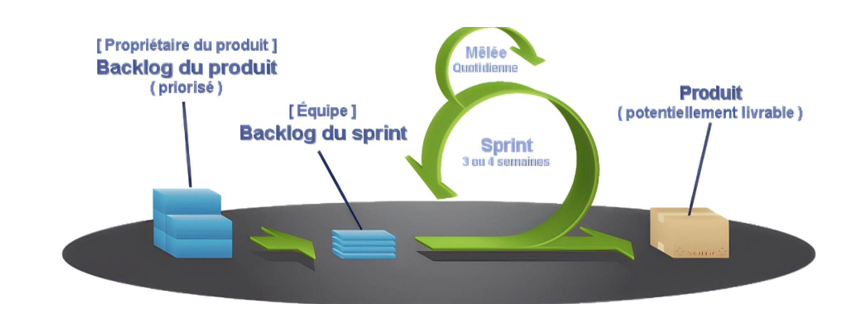
\includegraphics[width=14cm,height=6cm]{images/scrum.png}%
    }
\caption{Schéma illustratif de la méthodologie SCRUM}
\end{figure}
\vspace{-6mm}
\subsection{Justification du choix de SCRUM }
\vspace{-4mm}
Le recours à cette méthodologie est justifié uniquement lorsque SCRUM est utilisé pour garantir un produit de haute qualité, tout en respectant certains principes immuables tels que :\\
-	Tolérer tous les changements, même tardifs, apportés au cours du développement.\\
-	Livrer une application fonctionnelle.\\
-	Créer un projet autour de personnes motivées en leur fournissant un environnement et un soutien, et en leur faisant confiance.\\
-	Garantir un rythme de travail efficace.\\
-	Permettre aux membres de l'équipe de s'auto-organiser et de rechercher la simplicité.

\vspace{-7mm}

\section{Conclusion }
\vspace{-4mm}
Dans ce chapitre, nous avons introduit le cadre de notre stage en présentant l'entreprise d'accueil et en identifiant la problématique, suivie de la proposition d'une solution. Ensuite, nous avons exposé la méthode SCRUM que nous avons choisi d'adopter pour la réalisation de notre projet. Dans le chapitre suivant, nous allons procéder à l'analyse de l'outil \textbf{JIRA}.
    


\end{sloppypar}


 